\section{Applying Transport Classification Concept}

Considering if contaminant transport from the subsurface into the a building is dominated by advection or diffusion as it dramatically changes how a structure is expected to respond to change in pressurization; for diffusion dominated sites, contaminant entry rates will be relatively decoupled from building pressurization.
This has implications for a wide variety of VI topics, but perhaps most relevant for using CPM and choosing relevant ITS.\par

\subsection{Controlled Pressure Method}

The idea of CPM is to control the building pressurization, e.g. by using some fans or blowers, which in turn will control the contaminant entry rate.
The underlying assumption in its application is that contaminant entry into a building is largely advective in nature; for "diffusion sites" this will not be as effective.\par

Figure \ref{fig:cpm_adv_diff} illustrates this phenomena.
During the period when the land drain preferential pathway was open, CPM dramatically increased indoor contaminant concentrations compared to the when the CPM system was inactive.
However, after the closing of the land drain preferential pathway, CPM did not have any significant effect on indoor contaminant concentrations.
From the study of the ASU house and associated modeling explained it was deduced that the presence of the land drain preferential pathway make advection the dominant transport mechanism of contaminant vapors into the building.
This shows that CPM may not be universally effective, but could only reasonably expected to be so at "advection sites".\par

\begin{figure}[htb!]
  \centering
  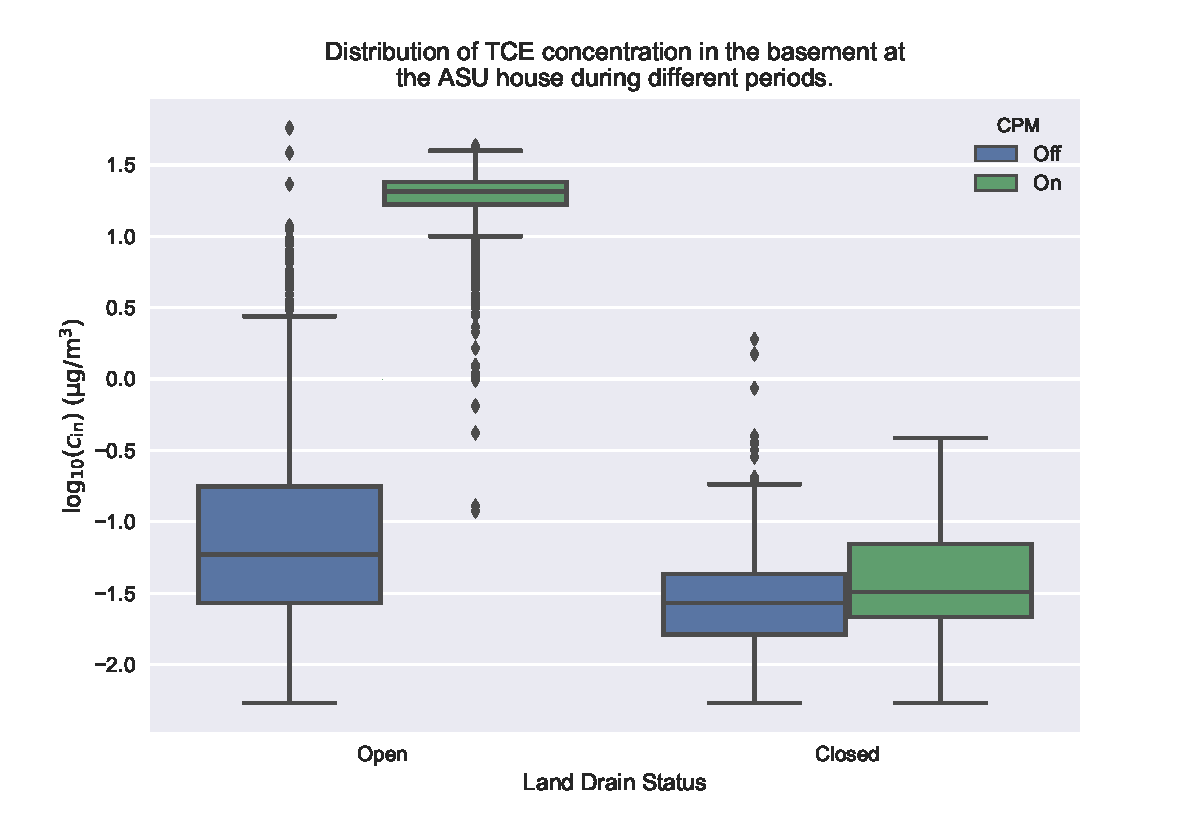
\includegraphics[width=0.75\textwidth]{asu_boxplot_concentration.pdf}
  \caption{Boxplot showing the log-10 transformed TCE concentrations at the ASU house. The CPM and natural periods, and the period before and after the land drain was closed are considered separately. The box signifies the interquartile range (IQR) of values, with the central line representing the median value, and the top and bottom of the box are the \nth{25} and \nth{75} percentiles. The whiskers extend to 1.5 times the IQR. Markers indicate outlier data points that fall outside the whiskers.}
  \label{fig:cpm_adv_diff}
\end{figure}

CPM not only affects the contaminant vapor entry rate into a building, but will also have an impact on air exchange rates.
Figure \ref{fig:asu_cpm_ae} shows the effect that CPM had on air exchange rates at the ASU house, where they increased significantly during the period.
The effect of this is that contaminant expulsion from the house is amplified, which decreases the indoor contaminant concentration for a given contaminant entry rate.
This is a concern voiced in \cite{holton_long-term_2015}\cite{holton_long-term_2015} evaluation of the CPM system at the ASU house, and suggested that a tracer-gas test to measure air exchange rate should be conducted during CPM.
This is used to introduce a correction term to account for the elevation of air exchange rate above its "natural" values.
Since CPM is used to determine the worst-case scenario, this correction term should be used to calculate the indoor contaminant concentration with worst-case entry rates, but "natural" air exchange rate values, i.e. $\approx \SI{0.5}{\per\hour}$ instead of the elevated values.\par

\begin{figure}[htb!]
  \centering
  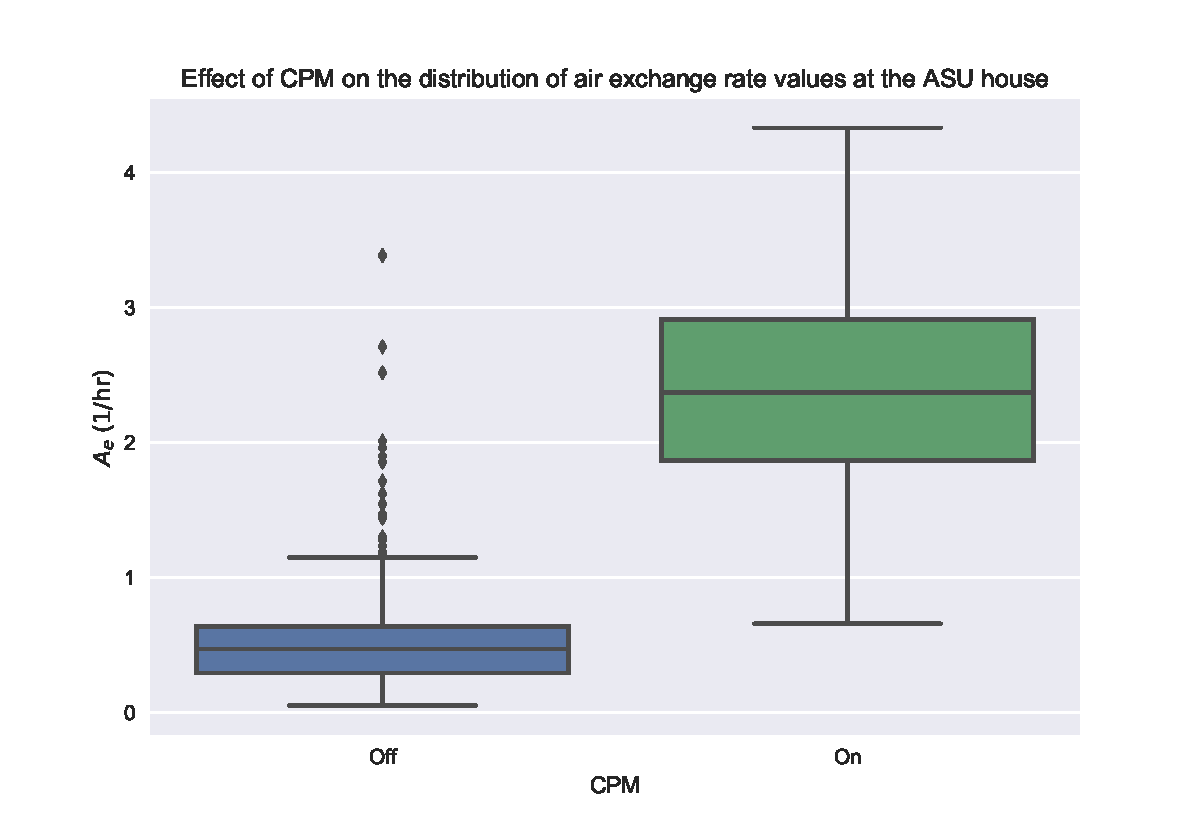
\includegraphics[width=0.75\textwidth]{asu_cpm_ae.pdf}
  \caption{Boxplot showing the distribution of air exchange rate values at the ASU house, considering the effect of CPM.}
  \label{fig:asu_cpm_ae}
\end{figure}

This highlights an issue with CPM at VI sites characterized by diffusive transport.
If the increased depressurization doesn't yield higher contaminant entry rates into the building, but elevates air exchange rate, then indoor contaminant concentration may be artificially lowered, and thus underdetermining the VI risk.
This further shows the necessity of using tracer-gas monitoring to measure air exchange rates when using CPM.\par

\subsection{Indicators, Tracers, And Surrogates}

As has been discussed throughout this work, VI can feature great temporal variability in indoor contaminant concentrations.
These variations can occur on a variety of time-scales, from days to larger seasonal trends, which can require significant amounts of data collection to fully resolve.
To reduce the resources expended on these efforts, and increase the likelihood of determining the relevant VI risk, it is desirable to use some indicators, tracers, and surrogates (ITS) that can be used to readily predict the periods and conditions when the highest indoor contaminant concentration at a site are likely to manifest.
Which specific ITS that are most appropriate for this task, and under which circumstances, are yet to be determined.\par

\begin{figure}[htb!]
  \centering
  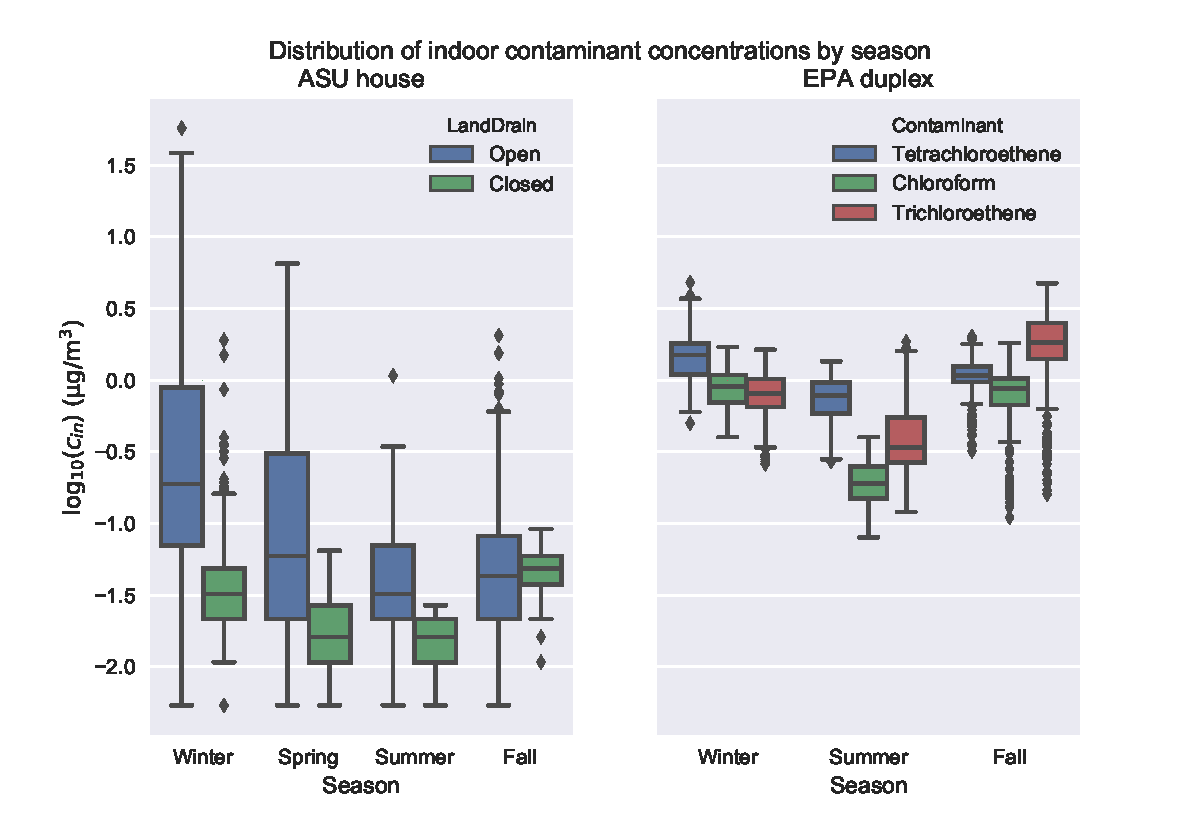
\includegraphics[width=\textwidth]{seasonal_concentration.pdf}
  \caption{Seasonal distribution of indoor contaminant concentration at the ASU house and EPA duplex. At the ASU house, the effect of the land drain preferential pathway is considered. At the EPA duplex, the differences in distribution for three different contaminants are considered. Here "winter" includes December to February, with each subsequent season being defined by the subsequent three months.}
  \label{fig:seasonal_concentration}
\end{figure}

Seasonal trends have been found to be common at many VI sites, with winter often cited as the period most likely to feature  elevated indoor contaminant concentrations\cite{burke_estimation_2010,hers_evaluation_2014,miles_temporal_2001,schumacher_fluctuation_2012,steck_indoor_2004}.
This is a trend that partly occurred at the ASU house as well (see Figure \ref{fig:seasonal_concentration}); indoor contaminant concentrations were highest during winter when the land drain preferential pathway was open, a trend was non-existent after the closing of the land drain.
At the EPA duplex, indoor contaminant concentrations were slightly higher during winter and fall than Summer, but only marginally so.\par

\begin{figure}[htb!]
  \centering
  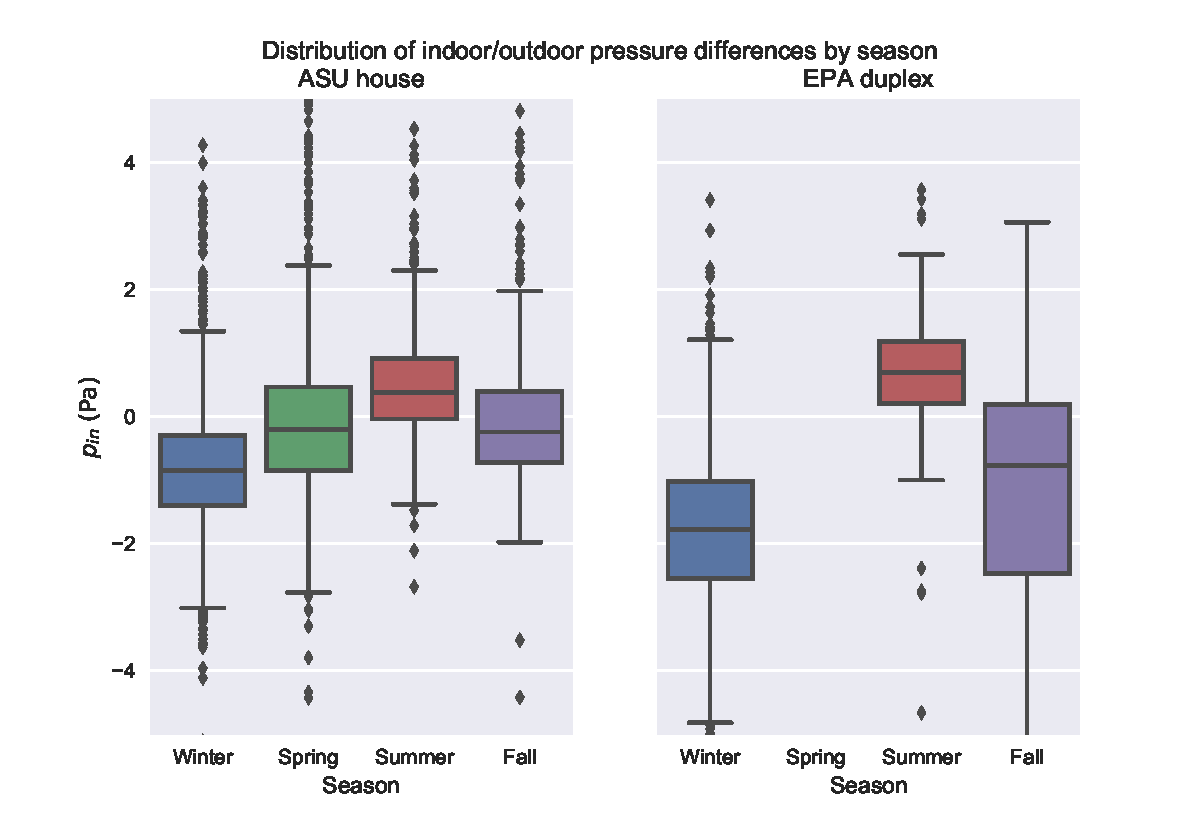
\includegraphics[width=\textwidth]{seasonal_pressure.pdf}
  \caption{Seasonal distribution of indoor contaminant concentration at the ASU house. A negative value indicates that the building is depressurized relative to ambient.}
  \label{fig:seasonal_pressure}
\end{figure}

The seasonal trend at the ASU house when the land drain preferential pathway was open, and its disappearance can be understood by examining the seasonal distribution of indoor/outdoor pressure difference values, in Figure \ref{fig:seasonal_pressure}.
Here we see that building depressurization is greatest during winter, slightly less depressurized during the shoulder seasons, and usually overpressurized during summer.
Putting this together with advective transport dominated period when the land drain preferential pathway was open at the ASU house, explains why indoor contaminant concentrations are higher during the colder seasons.
Conversely, when the land drain preferential pathway, contaminant transport was likely diffusion dominated, and such a trend disappears.\par

The EPA duplex exhibit a similar trend in building pressurization by season, i.e. it is more depressurized during colder seasons, and can help explain why indoor contaminant concentrations were likewise slightly higher during these seasons.
While the nature of the contaminant transport into the EPA duplex is not as well understood, it was showed in Chapter \ref{chp:preferential_pathways} that association between building pressurization and indoor contaminant concentrations were somewhere between that of the ASU house before and after the closing of the land drain (compare Figures \ref{fig:asu_pressure_dependence} and \ref{fig:indie_pressure_dependence}), indicating that while advection may not be dominant, it certainly isn't insignificant.\par

These data and analysis demonstrate that for advection sites, building pressurization could be used as an effective ITS, whereas at a diffusion site, it may not be.
However, to use building pressurization effectively as an ITS, it would be useful to be able to predict it based on some easier to measure parameters - such as weather conditions.\par
